\documentclass[dvipdfmx]{jarticle}

\usepackage{graphicx}
\usepackage{fullpage}
\usepackage{color}
\usepackage{ascmac}
\usepackage[dvipdfmx]{hyperref}
\usepackage{pxjahyper}
\usepackage{url}
\usepackage{comment}
\usepackage{ulem}
\usepackage{textcomp}

\begin{document}

%\thispagestyle{empty}

%\twocolumn[%
\begin{center}
\large\bf
\begin{tabular}{p{\textwidth}}
\hline
WSL(Windows Subsystem for Linux)環境の準備\hfill 吉田 光男\\
\hline
\end{tabular}
\end{center}
%\bigskip
%]{
%


\section{目的}

情報工学を学ぶ上で,プログラミングやUNIX/Linux/BSD環境の操作を経験することは避けられません.
プログラミングを試してみるだけであれば,Visual Studio\footnote{\url{https://visualstudio.microsoft.com/ja/}}やXcode\footnote{\url{https://developer.apple.com/jp/xcode/}}を導入するのも一つの方法です.
しかしこれらのツールは,主にWindowsまたはmacOSで作動するアプリケーションを開発することを目的としており,特定のプログラミング言語(C++,C\#,Swift)以外の開発には適していない場合があります.
また,特に研究開発の現場においては,UNIX/Linux/BSD環境での開発・実行を前提としている場合が多く,このような環境での操作に慣れておく必要もあるでしょう.

macOSはBSDをベースとして開発されたOSであり,ターミナル(端末エミュレータ)を立ち上げることで,UNIX/Linux/BSD環境を体験できます.
Windowsにはそのような環境が標準で用意されておらず,WSL(Windows Subsystem for Linux,Linux用Windowsサブシステム)を有効にした上で,UNIX/Linux/BSD環境を用意する必要があります.

本稿では,Windows 10を対象とし,WSLを有効にした上で,主要なLinuxディストリビューションの一つであるUbuntuをインストールする方法を説明します.
\textcolor{red}{なお,この作業では,多くの通信が発生します.
大学のWi-Fiを利用するなど,通信容量・速度に不安のない環境で行って下さい.}
また,事前にWindowsアップデートを実施し,Windows 10を最新の状態にして下さい.
Ubuntuのインストールには,5GB程度の空き容量が必要ですが,Ubuntuに様々なアプリケーションを導入する可能性を踏まえると,10GB以上の空き容量があることが望ましいでしょう.

\section{WSLの有効化とUbuntuのインストール}

WSL(Windows Subsystem for Linux,Linux用Windowsサブシステム)はマイクロソフト社が開発している仮想環境(のようなもの)です.
本稿では,簡略化したインストール手順のみを示すため,公式ドキュメント\footnote{\url{https://docs.microsoft.com/ja-jp/windows/wsl/}}も読むことをお勧めします.

WSLには,2021年3月現在,WSL 1とWSL 2の二つのバージョンがあります.
WSL 2の方が高度な機能を使えるものの,有効化の手順が複雑になるため,本稿ではWSL 1を使います.
なお,Windows 10のプレビュービルド(OSビルド20262以降,開発者向け)では,管理者特権のPowerShellにて,以下のコマンドを実行するだけでWSL 2 + Ubuntuの環境が整う\footnote{\url{https://docs.microsoft.com/ja-jp/windows/wsl/install-win10}}ことから,近い将来,同様に環境構築(\ref{sec:windows}と\ref{sec:ubuntu}の作業がコマンド一つで完了)できるようになるでしょう.
\begin{itembox}[l]{Windows PowerShell(管理者)}
\begin{verbatim}
wsl --install
\end{verbatim}
\end{itembox}

\subsection{WSL 1の有効化}\label{sec:windows}

まずは,WSLを有効化する必要があります.
この操作は,GUIまたはCUI(PowerShell)のいずれかで行えます(どちらか一方のみの作業で十分です).
いずれの作業を行った場合でも,設定を有効にするためにWindowsの再起動が必要になります.

GUIであれば,まず,スタート画面から「Windowsシステムツール」の中にある「コントロールパネル」を左クリックし,「プログラムと機能」を開きます.
このページの左側に「Windowsの機能の有効化または無効化」のリンクがあるので,これを左クリックします.
図\ref{fig:wsl}のような画面が表示されるので,「Linux用Windowsサブシステム」(環境によっては「Windows Subsystem for Linux」と表示されます)にチェックを入れて「OK」を左クリックします.

\begin{figure}[h]
  \centering
  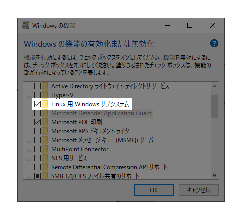
\includegraphics[width=0.6\linewidth]{figures/WSL.eps}
  \caption{Windows機能で「Linux用Windowsサブシステム」を有効にする}
  \label{fig:wsl}
\end{figure}

CUIであれば,まず,スタート画面から「Windows PowerShell」の中にある「Windows PowerShell」を\textcolor{red}{右}クリックし,「管理者として実行する」を左クリックします.
「ユーザアカウント制御」に付いて尋ねられるため,ここで「はい」を左クリックして,Windows PowerShellを管理者権限で立ち上げます.
ターミナル上で,以下のように入力し,実行(エンターキーを押す)します(図\ref{fig:PS}).
\begin{itembox}[l]{Windows PowerShell(管理者)}
\begin{verbatim}
Enable-WindowsOptionalFeature -Online -FeatureName Microsoft-Windows-Subsystem-Linux
\end{verbatim}
\end{itembox}

\begin{figure}[h]
  \centering
  \includegraphics[width=0.95\linewidth]{figures/PowerShell.png}
  \caption{Windows PowerShell(管理者)によるコマンド実行}
  \label{fig:PS}
\end{figure}

GUIまたはCUIでWSLを有効化した後,設定を反映させるためにWindowsを再起動します.

\subsection{Ubuntuのインストール}\label{sec:ubuntu}

WSLには様々なLinuxディストリビューションをインストールできますが,本稿では,一般的によく使われているUbuntuの最新版をインストールします.

まず,スタート画面から「Microsoft Store」を左クリックし,右上の「検索」を左クリックして「Ubuntu」を検索します.
図\ref{fig:store}のような画面が表示されるので,「Ubuntu」を左クリックした先のページで「入手」または「インストール」を左クリックします.
「サインインする方法」でアカウントを尋ねられた場合,適切なマイクロソフトアカウントでサインイン(ログイン)します.

\begin{figure}[h]
  \centering
  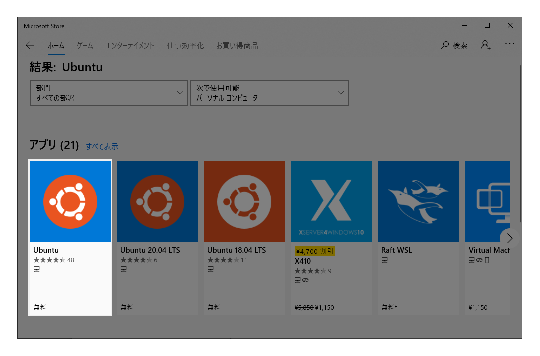
\includegraphics[width=0.95\linewidth]{figures/Store.eps}
  \caption{Microsoft Storeでの「Ubuntu」の検索結果}
  \label{fig:store}
\end{figure}

インストールが完了すると,「起動」のボタンが表示されるので,このボタンを左クリックします.
スタート画面から「Ubuntu」を左クリックしても,同様に起動できます.
Windowsアップデートと競合していると,エラーが発生する場合があります.
この場合,Windowsを再起動して下さい.

\subsection{Ubuntuの初期設定と作動確認}

スタート画面から「Ubuntu」を左クリックし,インストールしたUbuntuを起動します.
初回起動時には,図\ref{fig:Ubuntu}のように,ユーザ名(username)とパスワードを設定するように促されます.
ユーザ名は「user」のように,英数字一単語で設定します.
ここで設定するパスワードは,後述する「sudo」を使用する際に入力を求められます.
Windowsのパスワードと同じにする必要はありません.

\begin{figure}[h]
  \centering
  \includegraphics[width=0.95\linewidth]{figures/UbuntuDefault.png}
  \caption{Ubuntuの初期画面}
  \label{fig:Ubuntu}
\end{figure}

ユーザ名やパスワードの設定が終わったら,Ubuntuにインストールされているアプリケーション(パッケージ)を最新にする作業をしましょう.
UbuntuにはAPT(Advanced Package Tool)と呼ばれるパッケージ管理システムがあり,基本的に,アプリケーションの管理はAPTのコマンドを通じて行います.
インストールされているパッケージを最新にするには,以下のようにコマンドを入力します(図\ref{fig:AptUpdate}).
「\$」は一般ユーザ権限での実行を表すので,実際には入力不要です(画面上であらかじめ表示されています).
\begin{itembox}[l]{パッケージのアップデート}
\begin{verbatim}
$ sudo apt update
$ sudo apt upgrade
\end{verbatim}
\end{itembox}
「sudo」は後ろに続くコマンドを管理者権限(root)で実行するためのコマンドです.
「sudo」を実行する際には,「[sudo] password for XXX:」とユーザのパスワードが求められる場合があります.
この場合,初回起動時に設定したパスワードを入力します.
「apt upgrade」を実行すると,「Do you want to continue?」と尋ねられるので,エンターキーを押します(キャンセルする場合は「n」を入力してエンターキーを押します).

\begin{figure}[h]
  \centering
  \includegraphics[width=0.95\linewidth]{figures/UbuntuAptUpdate.png}
  \caption{sudo apt updateを実行した例}
  \label{fig:AptUpdate}
\end{figure}

「apt update」は,インストール可能なパッケージの一覧を更新します.
このコマンドだけでは,パッケージのインストールやアップグレードなどは行われません.
「apt upgrade」は,インストール済みのパッケージを最新のものに更新します.
この処理は,ローカルにあるパッケージの一覧を元に行われるため,パッケージを更新する際は,先に「apt update」を実行しておく必要があります.

\subsection{WindowsからUbuntuのファイルにアクセスする方法}\label{sec:file}

レポートの提出など,Ubuntuで作成したファイルをWindowsから参照したい場合があると思います.
Windowsからネットワークドライブ「\textbackslash\textbackslash{wsl}\$」にアクセスすることにより,WSL環境上のUbuntuのファイルにアクセスできます.
「\textbackslash」はバックスラッシュと呼ばれる記号で,Windowsの場合は「\textyen」のように表示される場合があります.
また,半角の「\textyen」を入力すれば,「\textyen」のように表示されていても,バックスラッシュ(\textbackslash)として機能します.

Windowsからファイルにアクセスできることを確認するために,まずは,以下を実行して空ファイルを作成しましょう(図\ref{fig:pwd}).
\begin{itembox}[l]{空ファイルの作成と確認}
\begin{verbatim}
$ touch sample.txt
$ pwd
$ ll
\end{verbatim}
\end{itembox}
「touch」は空ファイルを作成するコマンドで,今回はsample.txtという空ファイルを作成しています.
「pwd」は現在のディレクトリ(カレントディレクトリ)のパスを表示し,「ll」は現在のディレクトリにあるファイルの一覧を表示します.

\begin{figure}[h]
  \centering
  \includegraphics[width=0.95\linewidth]{figures/UbuntuPwd.png}
  \caption{空ファイルの作成と確認}
  \label{fig:pwd}
\end{figure}

次に,Windowsエクスプローラーを立ち上げ,図\ref{fig:explorer1}のようにアドレスバーに「\textbackslash\textbackslash{wsl}\$」を入力してエンターキーを押します.
エクスプローラーの立ち上げ方が分からない場合,スタート画面から「Windowsシステムツール」の中にある「エクスプローラー」を左クリックして下さい.

\begin{figure}[h]
  \centering
  
\includegraphics[width=0.95\linewidth]{figures/explorer1.eps}
  \caption{Windowsエクスプローラーのアドレスバーに「\textbackslash\textbackslash{wsl}\$」を入力}
  \label{fig:explorer1}
\end{figure}

\begin{figure}[h]
  \centering
  \includegraphics[width=0.95\linewidth]{figures/explorer2.png}
  \caption{Ubuntu → home → user とディレクトリを辿った例}
  \label{fig:explorer2}
\end{figure}

「Ubuntu」というネットワークドライブが見えるので,これをダブルクリックします.
その後,Ubuntuの「pwd」のコマンドで表示されたパス(例:「/home/user」)を辿ります.
具体的には,「home」をダブルクリックし,そして「user」をダブルクリックします.
すると,図\ref{fig:explorer2}のように,Ubuntuの「ll」のコマンドで表示されたファイルの一覧が表示されます.
Ubuntuで作成・編集したsample.txtはWindowsでアクセスできますし,Windowsでsample.txtを編集した場合,その結果はUbuntuにも反映されます.
つまり,WindowsとUbuntuでファイルが共有されています.

\subsection{Ubuntuのアンインストール}

Ubuntuのアンインストールは,ほかのWindowsアプリケーション同様に,設定の「アプリと機能」で行えます(図\ref{fig:WindowsApp}).
Ubuntuの環境が不要になった場合や環境を作り直す場合には,Ubuntuをアンインストールすると良いでしょう.
ただし,Ubuntuの中で作成したファイルも削除されるため,重要なファイルについては,\ref{sec:file}で説明したように,WindowsからUbuntuのファイルにアクセスし,別のディレクトリにコピーして下さい.

\begin{figure}[h]
  \centering
  \includegraphics[width=0.95\linewidth]{figures/WindowsApp.png}
  \caption{Ubuntuのアンインストール}
  \label{fig:WindowsApp}
\end{figure}


\section{Ubuntuの設定}

初期状態のUbuntuには,最低限のアプリケーション(パッケージ)しか入っていないため,プログラムを開発する環境としては不十分です.
まずは,プログラムを開発するのに必要な最低限のパッケージ(ビルドツール)をインストールしましょう.
以下のようにコマンドを入力します.
\begin{itembox}[l]{ビルドツールのインストール}
\begin{verbatim}
$ sudo apt update
$ sudo apt install build-essential
\end{verbatim}
\end{itembox}
このように,「apt install XXX」と実行することで,様々なパッケージを自動でインストールできます\footnote{\url{https://packages.ubuntu.com/ja/}}.
このインストール処理は,ローカルにあるパッケージの一覧を元に行われるため,インストールの際は,先に「apt update」を実行しておく必要があります.

以下を実行し,aptコマンドのマニュアルを表示してみましょう.
\begin{itembox}[l]{aptのマニュアルを確認}
\begin{verbatim}
$ man apt
\end{verbatim}
\end{itembox}
Ubuntuのコマンドで分からないことがあれば,まずはmanコマンドでマニュアルを読みましょう(qを押すことで終了できます).
インターネット上の解説は,コマンドのバージョンが異なるなどにより,正確でない場合もあります.

初期状態のUbuntuでは,ロケールが「C.UTF8」となっており,表示されるメッセージなどは英語です.
このままでも問題はありませんが,ロケールを「ja\_JP.UTF8」にし,表示されるメッセージなどを日本語にしたい場合は,以下のようにコマンドを入力します.
\begin{itembox}[l]{日本語言語パックのインストールとロケールの変更}
\begin{verbatim}
$ sudo apt update
$ sudo apt install language-pack-ja
$ sudo update-locale LANG=ja_JP.UTF8
\end{verbatim}
\end{itembox}
Ubuntuの再起動が必要になるため,以下のようにコマンドを入力し,Ubuntuを終了させます.
仮想環境上のUbuntuの再起動(一度終了させてからもう一度起動する)では,Windowsを再起動する必要はありません.
\begin{itembox}[l]{Ubuntuの終了}
\begin{verbatim}
$ exit
\end{verbatim}
\end{itembox}

ロケールを「ja\_JP.UTF8」にしたならば,Ubuntuを再起動した後,もう一度aptコマンドのマニュアルを表示してみましょう.
\begin{itembox}[l]{aptのマニュアルを確認}
\begin{verbatim}
$ man apt
\end{verbatim}
\end{itembox}
先ほどは英語のマニュアルが表示されましたが,今回は日本語のドキュメントが表示されるはずです.
また,同じコマンドを入力する場合,矢印キーの上(↑)を押すことで,過去のコマンドを辿ると,手間を省ける場合もあります.


\vspace{15mm}
以下では,先のビルドツール(build-essential)に加えて,授業で必要になる可能性のあるアプリケーション(パッケージ)のインストールの方法を説明します.
授業中にも指示がありますが,あらかじめ準備しておくと良いでしょう.

\subsection{B3:情報・知能工学実験(データサイエンス)}

日本語文を計算機に読み込ませるために,形態素解析器を導入します.
形態素解析器は,空白などの区切りのない日本語文を単語単位に分割するアプリケーションです.
今回,一般的によく使われるMeCab\footnote{\url{http://taku910.github.io/mecab/}}を利用します.
授業ではcurlも必要になりますが,これはビルドツールのインストールで導入済みです.

\begin{itembox}[l]{MeCabのインストール}
\begin{verbatim}
$ sudo apt update
$ sudo apt install mecab
\end{verbatim}
\end{itembox}

\begin{itembox}[l]{作動確認}
\begin{verbatim}
$ mecab -v
$ echo "本日は晴天なり" | mecab
$ echo "本日は晴天なり" | mecab -Owakati
$ curl --version
\end{verbatim}
\end{itembox}

MeCabを起動した場合,Ctrlを押しながらcを押すことで終了できます.
「curl」は外部からファイルをダウンロードするのに利用します.

\subsection{B3:ソフトウェア演習IV}

オブジェクト指向プログラミングのために,Javaの開発環境(JDK)を導入します.
授業ではgitも必要になりますが,これはビルドツールのインストールで導入済みです.

\begin{itembox}[l]{Javaのインストール}
\begin{verbatim}
$ sudo apt update
$ sudo apt install default-jdk
\end{verbatim}
\end{itembox}

\begin{itembox}[l]{作動確認}
\begin{verbatim}
$ java -version
$ javac -version
$ git --version
\end{verbatim}
\end{itembox}

「java」はJavaのプログラムを実行するために利用し,「javac」はJavaのソースコードをコンパイルする(プログラムに変換する)ために利用します.
「git」はソースコードをバージョン管理するために利用します.

\subsection{B3:プログラム言語論}

関数型プログラミングのために,CLISPとEmacsを導入します.
Emacsは主要なエディタの一つです.

\begin{itembox}[l]{CLISPとEmacsのインストール}
\begin{verbatim}
$ sudo apt update
$ sudo apt install clisp emacs
\end{verbatim}
\end{itembox}

\begin{itembox}[l]{作動確認}
\begin{verbatim}
$ clisp --version
$ emacs --version
\end{verbatim}
\end{itembox}

CLISPを起動した場合,「(exit)」と入力することで終了できます.
また,Emacsを起動した場合,Ctrlを押しながらxを押したあと,Ctrlを押しながらcを押すことで終了できます.

\subsection{M1:Webシステム特論}

Webシステムの構築演習のために,Node.jsを導入します.

\begin{itembox}[l]{Node.jsのインストール}
\begin{verbatim}
$ sudo apt update
$ sudo apt install nodejs
\end{verbatim}
\end{itembox}

\begin{itembox}[l]{作動確認}
\begin{verbatim}
$ nodejs -v
\end{verbatim}
\end{itembox}

Node.jsを起動した場合,「.exit」と入力することで終了できます.

\end{document}
